% A LaTeX (non-official) template for ISAE projects reports
% Copyright (C) 2014 Damien Roque

% This program is free software; you can redistribute it and/or
% modify it under the terms of the GNU General Public License
% as published by the Free Software Foundation; either version 2
% of the License, or (at your option) any later version.

% This program is distributed in the hope that it will be useful,
% but WITHOUT ANY WARRANTY; without even the implied warranty of
% MERCHANTABILITY or FITNESS FOR A PARTICULAR PURPOSE.  See the
% GNU General Public License for more details.

% You should have received a copy of the GNU General Public License
% along with this program; if not, write to the Free Software
% Foundation, Inc., 51 Franklin Street, Fifth Floor, Boston, MA  02110-1301, USA.

% Version: 0.2
% Author: Damien Roque <damien.roque_AT_isae.fr>

\documentclass[a4paper,12pt]{book}
\usepackage[utf8]{inputenc}
\usepackage[T1]{fontenc}
\usepackage[frenchb]{babel} % If you write in French
%\usepackage[english]{babel} % If you write in English
\usepackage{a4wide}
\usepackage{graphicx}
\graphicspath{{images/}}
\usepackage{subfig}
\usepackage{tikz}
\usetikzlibrary{shapes,arrows}
\usepackage{pgfplots}
\pgfplotsset{compat=newest}
\pgfplotsset{plot coordinates/math parser=false}
\newlength\figureheight
\newlength\figurewidth
\pgfkeys{/pgf/number format/.cd,
set decimal separator={,\!},
1000 sep={\,},
}
\usepackage{ifthen}
\usepackage{ifpdf}
\ifpdf
\usepackage[pdftex]{hyperref}
\else
\usepackage{hyperref}
\fi
\usepackage{color}
\hypersetup{%
colorlinks=true,
linkcolor=black,
citecolor=black,
urlcolor=black}

\renewcommand{\baselinestretch}{1.05}
\usepackage{fancyhdr}
\pagestyle{fancy}
\fancyfoot{}
\fancyhead[LE,RO]{\bfseries\thepage}
\fancyhead[RE]{\bfseries\nouppercase{\leftmark}}
\fancyhead[LO]{\bfseries\nouppercase{\rightmark}}
\setlength{\headheight}{15pt}

\let\headruleORIG\headrule
\renewcommand{\headrule}{\color{black} \headruleORIG}
\renewcommand{\headrulewidth}{1.0pt}
\usepackage{colortbl}
\arrayrulecolor{black}

\fancypagestyle{plain}{
  \fancyhead{}
  \fancyfoot[C]{\thepage}
  \renewcommand{\headrulewidth}{0pt}
}

\makeatletter
\def\@textbottom{\vskip \z@ \@plus 1pt}
\let\@texttop\relax
\makeatother

\makeatletter
\def\cleardoublepage{\clearpage\if@twoside \ifodd\c@page\else%
  \hbox{}%
  \thispagestyle{empty}%
  \newpage%
  \if@twocolumn\hbox{}\newpage\fi\fi\fi}
\makeatother

\usepackage{amsthm}
\usepackage{amssymb,amsmath,bbm}
\usepackage{array}
\usepackage{bm}
\usepackage{multirow}
\usepackage[footnote]{acronym}

\newcommand*{\SET}[1]  {\ensuremath{\mathbf{#1}}}
\newcommand*{\VEC}[1]  {\ensuremath{\boldsymbol{#1}}}
\newcommand*{\FAM}[1]  {\ensuremath{\boldsymbol{#1}}}
\newcommand*{\MAT}[1]  {\ensuremath{\boldsymbol{#1}}}
\newcommand*{\OP}[1]  {\ensuremath{\mathrm{#1}}}
\newcommand*{\NORM}[1]  {\ensuremath{\left\|#1\right\|}}
\newcommand*{\DPR}[2]  {\ensuremath{\left \langle #1,#2 \right \rangle}}
\newcommand*{\calbf}[1]  {\ensuremath{\boldsymbol{\mathcal{#1}}}}
\newcommand*{\shift}[1]  {\ensuremath{\boldsymbol{#1}}}

\newcommand{\eqdef}{\stackrel{\mathrm{def}}{=}}
\newcommand{\argmax}{\operatornamewithlimits{argmax}}
\newcommand{\argmin}{\operatornamewithlimits{argmin}}
\newcommand{\ud}{\, \mathrm{d}}
\newcommand{\vect}{\text{Vect}}
\newcommand{\sinc}{\ensuremath{\mathrm{sinc}}}
\newcommand{\esp}{\ensuremath{\mathbb{E}}}
\newcommand{\hilbert}{\ensuremath{\mathcal{H}}}
\newcommand{\fourier}{\ensuremath{\mathcal{F}}}
\newcommand{\sgn}{\text{sgn}}
\newcommand{\intTT}{\int_{-T}^{T}}
\newcommand{\intT}{\int_{-\frac{T}{2}}^{\frac{T}{2}}}
\newcommand{\intinf}{\int_{-\infty}^{+\infty}}
\newcommand{\Sh}{\ensuremath{\boldsymbol{S}}}
\newcommand{\C}{\SET{C}}
\newcommand{\R}{\SET{R}}
\newcommand{\Z}{\SET{Z}}
\newcommand{\N}{\SET{N}}
\newcommand{\K}{\SET{K}}
\newcommand{\reel}{\mathcal{R}}
\newcommand{\imag}{\mathcal{I}}
\newcommand{\cmnr}{c_{m,n}^\reel}
\newcommand{\cmni}{c_{m,n}^\imag}
\newcommand{\cnr}{c_{n}^\reel}
\newcommand{\cni}{c_{n}^\imag}
\newcommand{\tproto}{g}
\newcommand{\rproto}{\check{g}}
\newcommand{\LR}{\mathcal{L}_2(\SET{R})}
\newcommand{\LZ}{\ell_2(\SET{Z})}
\newcommand{\LZI}[1]{\ell_2(\SET{#1})}
\newcommand{\LZZ}{\ell_2(\SET{Z}^2)}
\newcommand{\diag}{\operatorname{diag}}
\newcommand{\noise}{z}
\newcommand{\Noise}{Z}
\newcommand{\filtnoise}{\zeta}
\newcommand{\tp}{g}
\newcommand{\rp}{\check{g}}
\newcommand{\TP}{G}
\newcommand{\RP}{\check{G}}
\newcommand{\dmin}{d_{\mathrm{min}}}
\newcommand{\Dmin}{D_{\mathrm{min}}}
\newcommand{\Image}{\ensuremath{\text{Im}}}
\newcommand{\Span}{\ensuremath{\text{Span}}}

\newtheoremstyle{break}
  {11pt}{11pt}%
  {\itshape}{}%
  {\bfseries}{}%
  {\newline}{}%
\theoremstyle{break}

%\theoremstyle{definition}
\newtheorem{definition}{Définition}[chapter]

%\theoremstyle{definition}
\newtheorem{theoreme}{Théorème}[chapter]

%\theoremstyle{remark}
\newtheorem{remarque}{Remarque}[chapter]

%\theoremstyle{plain}
\newtheorem{propriete}{Propriété}[chapter]
\newtheorem{exemple}{Exemple}[chapter]

\parskip=5pt
%\sloppy

\begin{document}

%%%%%%%%%%%%%%%%%%
%%% First page %%%
%%%%%%%%%%%%%%%%%%

\begin{titlepage}
\begin{center}


\includegraphics[width=0.5\textwidth]{enac}\\[1cm]

{\large IENAC15}\\[0.5cm]

{\large Rapport}\\[0.5cm]

% Title
\rule{\linewidth}{0.5mm} \\[0.4cm]
{ \huge \bfseries Topologie des architectures parallèles \\[0.4cm] }
\rule{\linewidth}{0.5mm} \\[1.5cm]

% Author and supervisor
\noindent
\begin{minipage}{0.4\textwidth}
  \begin{flushleft} \large
    \emph{Auteurs :}\\
    M. Florian \textsc{Barbarin}\\
    M. Nicolas \textsc{Holvoet}\\
%    M\up{me} Prénom \textsc{Nom}\\
    M. Abdelkader \textsc{Beldjilali}
  \end{flushleft}
\end{minipage}%
\begin{minipage}{0.4\textwidth}
 \begin{flushright} \large
   \emph{Encadrants :} \\
   M. Stéphane \textsc{Puechmorel}\\
   M. Rémi \textsc{Coudarcher}
 \end{flushright}
\end{minipage}

\vfill

% Bottom of the page
{\large Version 0.1 du\\ \today}

\end{center}
\end{titlepage}

%%%%%%%%%%%%%%%%%%%%%%%%%%%%%
%%% Non-significant pages %%%
%%%%%%%%%%%%%%%%%%%%%%%%%%%%%

\frontmatter

% \chapter*{Remerciements}
% Lorem ipsum dolor sit amet, consectetur adipiscing elit. Sed non risus. Suspendisse lectus tortor, dignissim sit amet, adipiscing nec, ultricies sed, dolor. Cras elementum ultrices diam. Maecenas ligula massa, varius a, semper congue, euismod non, mi. Proin porttitor, orci nec nonummy molestie, enim est eleifend mi, non fermentum diam nisl sit amet erat. Duis semper. Duis arcu massa, scelerisque vitae, consequat in, pretium a, enim. Pellentesque congue. Ut in risus volutpat libero pharetra tempor. Cras vestibulum bibendum augue. Praesent egestas leo in pede. Praesent blandit odio eu enim. Pellentesque sed dui ut augue blandit sodales. Vestibulum ante ipsum primis in faucibus orci luctus et ultrices posuere cubilia Curae; Aliquam nibh. Mauris ac mauris sed pede pellentesque fermentum. Maecenas adipiscing ante non diam sodales hendrerit. Ut velit mauris, egestas sed, gravida nec, ornare ut, mi. Aenean ut orci vel massa suscipit pulvinar. Nulla sollicitudin. Fusce varius, ligula non tempus aliquam, nunc turpis ullamcorper nibh, in tempus sapien eros vitae ligula. Pellentesque rhoncus nunc et augue. Integer id felis.
% 
% \clearpage
% \tableofcontents
% 
% \clearpage
% \listoffigures
% 
% \clearpage
% \chapter*{Liste des sigles et acronymes}
% \begin{acronym}[CP-OFDMX] % Give the longest acronym here
% \acro{ASK}{\emph{Amplitude Shift Keying}}
% \acro{AWGN}{\emph{Additive White Gaussian Noise}}
% \acro{BABG}{Bruit Additif Blanc Gaussien}
% \acro{BCJR}{\emph{Bahl, Cocke, Jelinek, Raviv}}
% \acro{BER}{\emph{Binary Error Rate}}
% \acro{BFDM}{\emph{Biorthogonal Frequency Division Multiplexing}}
% \end{acronym}

%%%%%%%%%%%%%%%%%%%%%%%%%%%%%%%%%%%%%%%%%%%%
%%% Content of the report and references %%%
%%%%%%%%%%%%%%%%%%%%%%%%%%%%%%%%%%%%%%%%%%%%

\mainmatter
\pagestyle{fancy}

\cleardoublepage

%\chapter*{Introduction}
\addcontentsline{toc}{chapter}{Introduction}
\markboth{Introduction}{Introduction}
\label{chap:introduction}
%\minitoc

Lorem ipsum dolor sit amet, consectetur adipiscing elit. Sed non risus. Suspendisse lectus tortor, dignissim sit amet, adipiscing nec, ultricies sed, dolor. Cras elementum ultrices diam. Maecenas ligula massa, varius a, semper congue, euismod non, mi. Proin porttitor, orci nec nonummy molestie, enim est eleifend mi, non fermentum diam nisl sit amet erat. Duis semper. Duis arcu massa, scelerisque vitae, consequat in, pretium a, enim. Pellentesque congue. Ut in risus volutpat libero pharetra tempor. Cras vestibulum bibendum augue. Praesent egestas leo in pede. Praesent blandit odio eu enim. Pellentesque sed dui ut augue blandit sodales. Vestibulum ante ipsum primis in faucibus orci luctus et ultrices posuere cubilia Curae; Aliquam nibh. Mauris ac mauris sed pede pellentesque fermentum. Maecenas adipiscing ante non diam sodales hendrerit. Ut velit mauris, egestas sed, gravida nec, ornare ut, mi. Aenean ut orci vel massa suscipit pulvinar. Nulla sollicitudin. Fusce varius, ligula non tempus aliquam, nunc turpis ullamcorper nibh, in tempus sapien eros vitae ligula. Pellentesque rhoncus nunc et augue. Integer id felis. Curabitur aliquet pellentesque diam. Integer quis metus vitae elit lobortis egestas. Lorem ipsum dolor sit amet, consectetuer adipiscing elit. Morbi vel erat non mauris convallis vehicula. Nulla et sapien. Integer tortor tellus, aliquam faucibus, convallis id, congue eu, quam. Mauris ullamcorper felis vitae erat. Proin feugiat, augue non elementum posuere, metus purus iaculis lectus, et tristique ligula justo vitae magna. Aliquam convallis sollicitudin purus. Praesent aliquam, enim at fermentum mollis, ligula massa adipiscing nisl, ac euismod nibh nisl eu lectus. Fusce vulputate sem at sapien. Vivamus leo. Aliquam euismod libero eu enim. Nulla nec felis sed leo placerat imperdiet. Aenean suscipit nulla in justo. Suspendisse cursus rutrum augue. Nulla tincidunt tincidunt mi. Curabitur iaculis, lorem vel rhoncus faucibus, felis magna fermentum augue, et ultricies lacus lorem varius purus. Curabitur eu amet.

Lorem ipsum dolor sit amet, consectetur adipiscing elit. Sed non risus. Suspendisse lectus tortor, dignissim sit amet, adipiscing nec, ultricies sed, dolor. Cras elementum ultrices diam. Maecenas ligula massa, varius a, semper congue, euismod non, mi. Proin porttitor, orci nec nonummy molestie, enim est eleifend mi, non fermentum diam nisl sit amet erat. Duis semper. Duis arcu massa, scelerisque vitae, consequat in, pretium a, enim. Pellentesque congue. Ut in risus volutpat libero pharetra tempor. Cras vestibulum bibendum augue. Praesent egestas leo in pede. Praesent blandit odio eu enim. Pellentesque sed dui ut augue blandit sodales. Vestibulum ante ipsum primis in faucibus orci luctus et ultrices posuere cubilia Curae; Aliquam nibh. Mauris ac mauris sed pede pellentesque fermentum. Maecenas adipiscing ante non diam sodales hendrerit. Ut velit mauris, egestas sed, gravida nec, ornare ut, mi. Aenean ut orci vel massa suscipit pulvinar. Nulla sollicitudin. Fusce varius, ligula non tempus aliquam, nunc turpis ullamcorper nibh, in tempus sapien eros vitae ligula. Pellentesque rhoncus nunc et augue. Integer id felis. Curabitur aliquet pellentesque diam. Integer quis metus vitae elit lobortis egestas. Lorem ipsum dolor sit amet, consectetuer adipiscing elit. Morbi vel erat non mauris convallis vehicula. Nulla et sapien. Integer tortor tellus, aliquam faucibus, convallis id, congue eu, quam. Mauris ullamcorper felis vitae erat. Proin feugiat, augue non elementum posuere, metus purus iaculis lectus, et tristique ligula justo vitae magna. Aliquam convallis sollicitudin purus. Praesent aliquam, enim at fermentum mollis, ligula massa adipiscing nisl, ac euismod nibh nisl eu lectus. Fusce vulputate sem at sapien. Vivamus leo. Aliquam euismod libero eu enim. Nulla nec felis sed leo placerat imperdiet. Aenean suscipit nulla in justo. Suspendisse cursus rutrum augue. Nulla tincidunt tincidunt mi. Curabitur iaculis, lorem vel rhoncus faucibus, felis magna fermentum augue, et ultricies lacus lorem varius purus. Curabitur eu amet.

%%% Local Variables: 
%%% mode: latex
%%% TeX-master: "isae-report-template"
%%% End: 

\chapter{Graphes et topologie de réseaux}
\label{chap:premierchapitre}

\section{Algorithme de Dijkstra}
Edgser Wybe Dijkstra (EWD), Physicien Néerlandais reconverti à l'informatique en 1955, a proposé en 1959 un algorithme de recherche de chemin minimum 
dans un graphe  dont  la complexité est en O(n). 

\begin{figure}[htp]
  \centering
  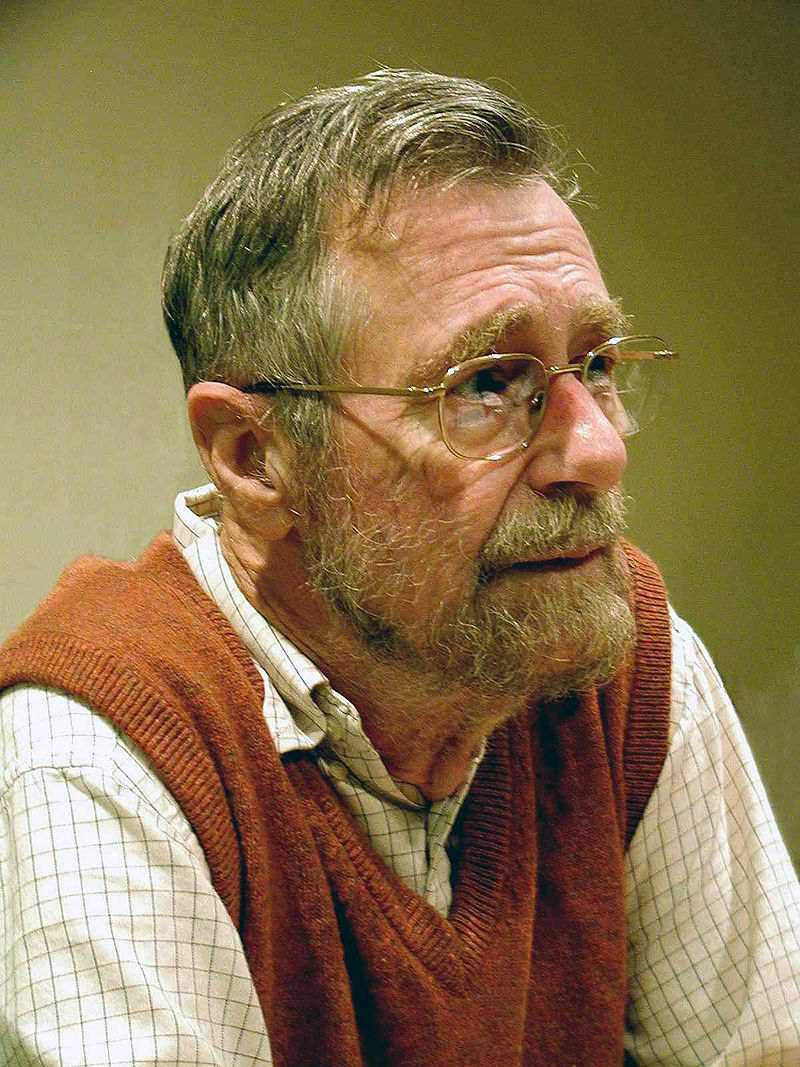
\includegraphics[width=4cm]{images/Edsger_Wybe_Dijkstra}
  \caption{Edgser Wybe Dijkstra (1930-2002)}
  \label{fig:une-autre-image}
\end{figure}

On doit à Dijkstra, qui avait la réputation d'avoir mauvais caractère et de présenter une allergie au ``GOTO'',
quelques citations\footnote{source : \url{https://fr.wikipedia.org/wiki/Edsger_Dijkstra}} telles que :


\begin{quote}
\textit{« Il est pratiquement impossible d'enseigner la bonne programmation aux étudiants 
qui ont eu une exposition antérieure au BASIC : comme programmeurs potentiels, 
ils sont mentalement mutilés, au-delà de tout espoir de régénération. »}
\end{quote}

\begin{quote}
\textit{« Le plus court chemin d'un graphe n'est jamais celui que l'on croit, 
il peut surgir de nulle part, et la plupart du temps, il n'existe pas. »}
\end{quote}

\begin{quote}
\textit{« La programmation par objets est une idée exceptionnellement mauvaise qui ne pouvait naître qu'en Californie. »}
\end{quote}


L'algorithme donne le plus court chemin de la source à \textit{tous les sommets} d'un graphe 
connexe pondéré (orienté ou non) dont le poids lié aux arêtes est positif ou nul.



 %\cite{Roque2012,Roque2012b,Roque2012c,Roque2012d}. 
 


\begin{figure}[htp]
  \centering
  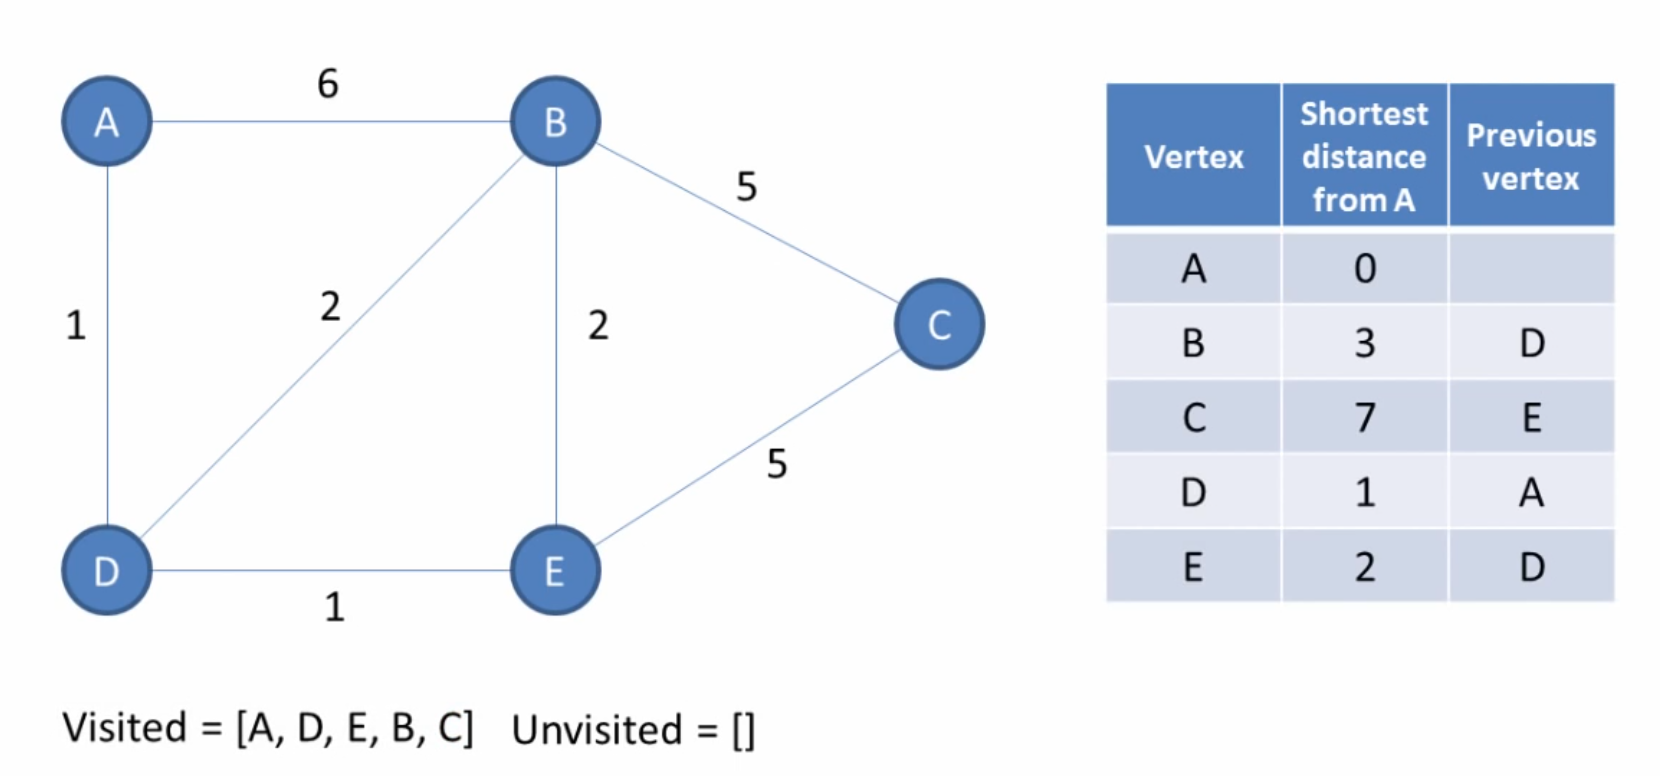
\includegraphics[width=15cm]{images/algo_dij}
  \caption{Exemple de calcul des plus courts chemins à partir du noeud A.}
  \label{fig:une-autre-image}
\end{figure}

L'algorithme de Disjkstra est un algorithme glouton qui utilise l'hypothèse qu'une décision prise sur la base
d'un critère d'optimalité locale conduira à un optimum global. Ainsi, à chaque itération, l'algorithme choisit le noeud
du réseau dont la distance au noeud de départ est la plus faible.
% \begin{figure}[htp]
%   \centering
%   \tikzstyle{block} = [draw, fill=blue!20, rectangle, minimum height=3em, minimum width=6em, text width=6em,text centered]
\begin{tikzpicture}[auto, node distance=3.5cm,>=latex']
\shorthandoff{:} % Evite le bug de compilation avec tikz
    % Longueurs et espacement
    \def\longabove{0.2cm}
    \def\espacement{4cm}

    % Définition des blocs
    \node [block, node distance=\espacement] (codeur) {Codeur};
    \node [block, right of=codeur, node distance=\espacement] (cbs) {CBS};
    \node [block, right of=cbs, node distance=\espacement] (modulateur) {Modulateur};
 
    % Définition des liens
    \draw [<-] (codeur) -- ++(-2,0) node[left] {$\{b_n\}$};
    \draw [->] (codeur) -- node[above=\longabove] {$\{d_n\}$} (cbs);
    \draw [->] (cbs) -- node[above=\longabove] {$\{c_k\}$} (modulateur);
    \draw [->] (modulateur) -- ++(2,0) node[right] {$s(t)$};
\end{tikzpicture}

%   \caption{Exemple de diagramme TikZ.}
%   \label{fig:une-image}
% \end{figure}

\section{Algorithme A*}
Lorem ipsum dolor sit amet, consectetur adipiscing elit. Sed non risus. Suspendisse l
\section{Utilisation}

Dijkstra est utilisé dans le routaghe dynamique OSPF
Comment les utiliser pour transférer de façon optimale une donnée d'un noeud à un autre. 

\begin{table}[ht]
  \begin{center}
    \begin{tabular}{|c|c|c|c|c|}
      \hline
      & $h(t,\tau)$ & $S_{\OP{H}}^{(\alpha)} (f,\tau)$ & $L_{\OP{H}}^{(\alpha)} (\nu,t)$ & $H^{(\alpha)}(f,\nu)$ \\
      \hline
      LTI & $q(\tau)$ & $q(\tau) \delta(f)$ & $Q(\nu)$ & $Q(\nu) \delta(\nu-f)$ \\
      \hline
      LFI & $m(t) \delta(\tau)$ & $M(f) \delta(\tau)$ & $m(t)$ & $M(f)$\\
      \hline
      identité & $\delta(t)$ & $\delta(f)\delta(\tau)$ & $1$ & $\delta(\nu-f)$\\
      \hline
    \end{tabular}
    \caption{Exemple de tableau.}
    \label{tab:un-tableau}
  \end{center}
\end{table}

Lorem ipsum dolor sit amet, consectetur adipiscing elit. Sed non risus. Suspendisse lectus tortor, dignissim sit amet, adipiscing nec, ultricies sed, dolor. Cras elementum ultrices diam. Maecenas ligula massa, varius a, semper congue, euismod non, mi. Proin porttitor, orci nec nonummy molestie, enim est eleifend mi, non fermentum diam nisl sit amet erat. Duis semper. Duis arcu massa, scelerisque vitae, consequat in, pretium a, enim. Pellentesque congue. Ut in risus volutpat libero pharetra tempor. Cras vestibulum bibendum augue. Praesent egestas leo in pede. Praesent blandit odio eu enim. Pellentesque sed dui ut augue blandit sodales. Vestibulum ante ipsum primis in faucibus orci luctus et ultrices posuere cubilia Curae; Aliquam nibh. Mauris ac mauris sed pede pellentesque fermentum. Maecenas adipiscing ante non diam sodales hendrerit. Ut velit mauris, egestas sed, gravida nec, ornare ut, mi. Aenean ut orci vel massa suscipit pulvinar. Nulla sollicitudin. Fusce varius, ligula non tempus aliquam, nunc turpis ullamcorper nibh, in tempus sapien eros vitae ligula. Pellentesque rhoncus nunc et augue. Integer id felis. Curabitur aliquet pellentesque diam. Integer quis metus vitae elit lobortis egestas. Lorem ipsum dolor sit amet, consectetuer adipiscing elit. Morbi vel erat non mauris convallis vehicula. Nulla et sapien. Integer tortor tellus, aliquam faucibus, convallis id, congue eu, quam. Mauris ullamcorper felis vitae erat. Proin feugiat, augue non elementum posuere, metus purus iaculis lectus, et tristique ligula justo vitae magna. Aliquam convallis sollicitudin purus. Praesent aliquam, enim at fermentum mollis, ligula massa adipiscing nisl, ac euismod nibh nisl eu lectus. Fusce vulputate sem at sapien. Vivamus leo. Aliquam euismod libero eu enim. Nulla nec felis sed leo placerat imperdiet. Aenean suscipit nulla in justo. Suspendisse cursus rutrum augue. Nulla tincidunt tincidunt mi. Curabitur iaculis, lorem vel rhoncus faucibus, felis magna fermentum augue, et ultricies lacus lorem varius purus. Curabitur eu amet (fig. \ref{fig:une-autre-image}).

\begin{figure}[htp]
  \centering
  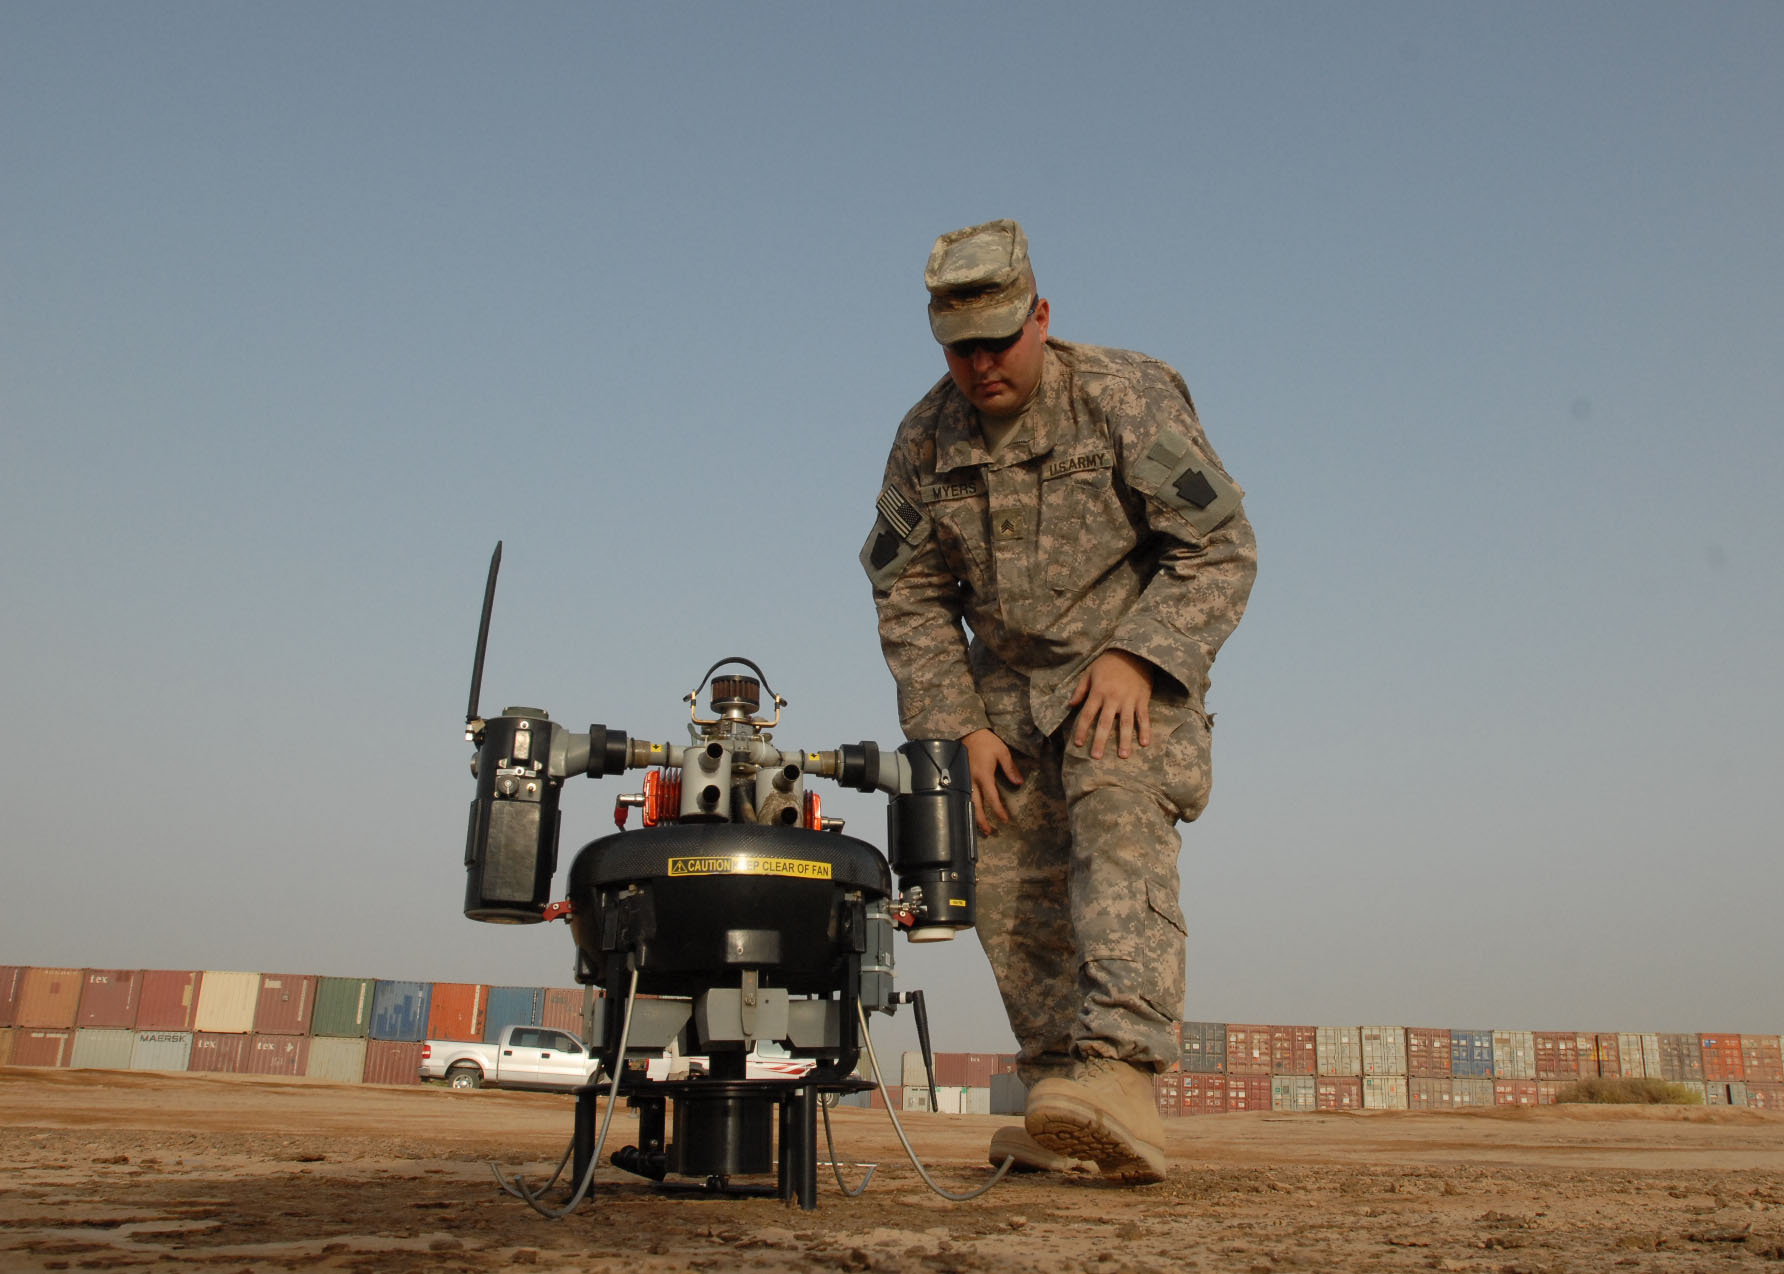
\includegraphics[width=4cm]{images/bitmap_image}
  \caption{Exemple d'image au format JPG.}
  \label{fig:une-autre-image}
\end{figure}


%%% Local Variables: 
%%% mode: latex
%%% TeX-master: "isae-report-template"
%%% End: 
\section{Les grilles}

\subsection{Défintion}

\begin{dfn}
Une grille de dimension $d$ possédant $N$ nœuds suivant chaque coordonnée est le produit cartésien de $d$ chaines ($d>1$) de $N$ sommets. On note cette grille $M(N)^d$ que l'on dira \textit{de coté N}.
\end{dfn}




\begin{rem}

Si l'on considère le produit cartésien de deux graphes, le graphe résultant est tel que :
\begin{itemize}
\item l'ensemble de ses nœuds est le produit cartésien des nœuds des deux premiers graphes;
\item deux de ses nœuds sont voisins s'ils sont composés de nœuds qui étaient voisins dans l'un des deux premiers graphes.
\end{itemize}

\end{rem}

\begin{ex}

Soient deux chaines composées des nœuds appartenant à l'ensemble $E = \{A, B, C, D\}$. Le produit cartésien de ces deux chaines ($d=2$) de taille $N = Card(E) = 4$ :

\begin{center}

\begin{minipage}[c]{.5\linewidth}
\begin{minipage}[c]{.2\linewidth}

\begin{tikzpicture}
\SetGraphUnit{1}
\GraphInit[vstyle=Normal]
\Vertex{A}
\EA(A){B} \EA(B){C} \EA(C){D}
\Edges[color=red](A,B,C,D)
\end{tikzpicture}
\end{minipage}
\hfill
\begin{minipage}[c]{.2\linewidth}
\begin{tikzpicture}
\SetGraphUnit{1}
\GraphInit[vstyle=Normal]
\Vertex{A}
\SO(A){B} \SO(B){C} \SO(C){D}
\Edges(A,B,C, D)
\end{tikzpicture}

\end{minipage}
\end{minipage}
\end{center}

A pour résultat la grille $M(4)^2$  : 

\begin{center}
\begin{minipage}[c]{.2\linewidth}
\begin{tikzpicture}
\SetGraphUnit{1.2}
\GraphInit[vstyle=Normal]
\Vertex{AA}
\EA(AA){BA} \EA(BA){CA} \EA(CA){DA}
\SO(AA){AB}
\EA(AB){BB} \EA(BB){CB} \EA(CB){DB}
\SO(AB){AC}
\EA(AC){BC} \EA(BC){CC} \EA(CC){DC}
\SO(AC){AD}
\EA(AD){BD} \EA(BD){CD} \EA(CD){DD}

\Edges(AA,BA,CA,DA)
\Edges(AB,BB,CB,DB)
\Edges(AC,BC,CC,DC)
\Edges(AD,BD,CD,DD)

\Edges(AA,AB,AC,AD)
\Edges(BA,BB,BC,BD)
\Edges(CA,CB,CC,CD)
\Edges(DA,DB,DC,DD)
\end{tikzpicture}
\end{minipage}
\end{center}

\end{ex}

\subsection{Propriétés}

\subsubsection*{Nombre total de nœuds}



Il résulte de la définition ci-dessus que le nombre total de nœuds est égal au cardinal du produit cartésien de l'ensemble des nœuds de départ :

$$Card(S)= Card(\underbrace{E \times E \times ... \times E}_{\text{p fois}}) = \prod_1^p Card(E) = N^p$$

$$\text{où } S \text{ est l'ensemble des noeuds de la grille}$$

\subsubsection*{Nombre total d'arêtes}

Soit $A$ l'ensemble des arêtes de la grille. Voici pour $N=2$ et $N=4$ le passage de la dimension $1$ aux dimensions supérieures ($2$ et $3$).


\begin{center}

\begin{tabular}{cccccc}

&$d = 1$ & & $d = 2$ & & $d = 3$\\ 

$N=2$& 

\begin{minipage}[c]{0.2\linewidth}
\begin{center}
\begin{tikzpicture}
\SetGraphUnit{1}
\GraphInit[vstyle=Normal]
\Vertex{A}
\EA(A){B}
\Edges[color=blue](A,B)
\end{tikzpicture}
\end{center}
\end{minipage} 

& $\longrightarrow$ & 

\begin{minipage}[c]{0.2\linewidth}
\begin{center}
\begin{tikzpicture}
\SetGraphUnit{1.2}
\GraphInit[vstyle=Normal]
\Vertex{AA}
\EA(AA){BA}
\SO(AA){AB}
\EA(AB){BB}


\Edges(AA,BA,BB,AB,AA)

\end{tikzpicture}
\end{center}
\end{minipage}
 
& $\longrightarrow$ &

\begin{minipage}[c]{0.2\linewidth}
\begin{center}
\resizebox{3cm}{3cm}{
\begin{tikzpicture}
\SetGraphUnit{2}
\GraphInit[vstyle=Normal]
\Vertex{AAA}
\EA(AAA){BAA}
\SO(AAA){ABA}
\EA(ABA){BBA}
\Vertex[x=1 , y=1]{AAB}
\EA(AAB){BAB}
\SO(AAB){ABB}
\EA(ABB){BBB}


\Edges(AAA,BAA,BBA,ABA,AAA)
\Edges(AAA,AAB,BAB,BAA)
\Edges(ABA,ABB,BBB,BBA)
\Edges(AAB,ABB)
\Edges(BAB,BBB)

\end{tikzpicture}}
\end{center}
\end{minipage}

\\ 

 & $Card(A) = 1$ & & $Card(A) = 4$ & & $Card(A) = 12$ \\
 &  & & & & \\

$N = 3$ &

\begin{minipage}[c]{0.2\linewidth}
\begin{center}
\begin{tikzpicture}
\SetGraphUnit{1}
\GraphInit[vstyle=Normal]
\Vertex{A}
\EA(A){B} \EA(B){C}
\Edges(A,B,C)
\end{tikzpicture}
\end{center}
\end{minipage}

&
$\longrightarrow$
& 
\begin{minipage}[c]{0.2\linewidth}
\begin{center}
\begin{tikzpicture}
\SetGraphUnit{1.2}
\GraphInit[vstyle=Normal]
\Vertex{AA}
\EA(AA){BA} \EA(BA){CA}
\SO(AA){AB}
\EA(AB){BB} \EA(BB){CB}
\SO(AB){AC}
\EA(AC){BC} \EA(BC){CC}


\Edges(AA,BA,CA)
\Edges(AB,BB,CB)
\Edges(AC,BC,CC)

\Edges(AA,AB,AC)
\Edges(BA,BB,BC)
\Edges(CA,CB,CC)
\end{tikzpicture}
\end{center}
\end{minipage}

& $\longrightarrow$ &

\begin{minipage}[c]{0.2\linewidth}
\begin{center}
\resizebox{3.5cm}{3.5cm}{
\begin{tikzpicture}
\GraphInit[vstyle=Normal]
\SetGraphUnit{2.5}
%\draw[help lines] (0,-3) grid (2,2);

\Vertex[x=2 , y=-3]{ACC}
\EA(ACC){BCC} \EA(BCC){CCC}
\Edges(ACC,BCC,CCC)

\Vertex[x=1 , y=-4]{ACB}
\EA(ACB){BCB} \EA(BCB){CCB}
\Edges(ACB,BCB,CCB)

\Vertex[x=2 , y=-0.5]{ABC}
\EA(ABC){BBC} \EA(BBC){CBC}
\Edges(ABC,BBC,CBC)

\Vertex[x=1 , y=-1.5]{ABB}
\EA(ABB){BBB} \EA(BBB){CBB}
\Edges(ABB,BBB,CBB)

\Vertex[x=2 , y=2]{AAC}
\EA(AAC){BAC} \EA(BAC){CAC}
\Edges(AAC,BAC,CAC)

\Vertex[x=1 , y=1]{AAB}
\EA(AAB){BAB} \EA(BAB){CAB}
\Edges(AAB,BAB,CAB)

\Vertex{AAA}
\EA(AAA){BAA} \EA(BAA){CAA}
\Edges(AAA,BAA,CAA)

\SO(AAA){ABA} \EA(ABA){BBA} \EA(BBA){CBA}

\SO(ABA){ACA} \EA(ACA){BCA} \EA(BCA){CCA}
\Edges(ABA,ABB,ABC)
\Edges(BBA,BBB,BBC)
\Edges(CBA,CBB,CBC)
\Edges(AAA,AAB,AAC)
\Edges(BAA,BAB,BAC)
\Edges(CAA,CAB,CAC)
\Edges(ABA,BBA,CBA)
\Edges(ACA,BCA,CCA)
\Edges(AAA, ABA, ACA,ACA,ACB,ACC, ABC, AAC)
\Edges(BAA, BBA,BCA,BCB,BCC,BBC, BAC)
\Edges(CAA, CBA, CCA,CCB,CCC, CBC, CAC)
\Edges(CAB,CBB,CCB)
\Edges(BAB,BBB,BCB)
\Edges(AAB,ABB,ACB)
\end{tikzpicture}
}
\end{center}
\end{minipage}\\

 & $Card(A) = 2$ & & $Card(A) = 12$ & & $Card(A) = 54$ \\


\end{tabular}

\end{center}

On remarque à présent que, pour $N$ fixé, le passage d'une dimension $d$ à une dimension $d+1$ se fait en deux étapes :
\begin{itemize}
\item on "copie" $N$ fois la grille de dimension $d$;
\item on relie, par une arête, les nœuds de la grille $1$ avec les nœuds correspondants de la grille $2$ puis les nœuds de la grille $2$ avec les nœuds correspondants de la grille $3$, et ainsi de suite jusqu'à la grille $N$.
\end{itemize}

Cette méthode de construction nous donne une relation de récurrence pour le nombre d'arêtes : 

$$Card(A)_{d+1} = \underbrace{N \times Card(A)_d}_{\text{On copie }N\text{ fois la grille de dimension }d} + \underbrace{(N-1)\times Card(S)_d}_{\text{On relie les arêtes de chaque grille}}$$

On ne peut aisément déterminer une expression générale de la suite ci-dessus. Or les exemples précédents nous permettent de déduire une expression du nombre d'arêtes en fonction de $d$ et de $N$ : 

$$Card(A)_d = d\times (N-1)\times N^{d-1}$$

Nous pouvons démontrer par récurrence cette expression.

\begin{proof}[Preuve de la relation]
\item
\paragraph{Initialisation :} 
Pour $d=1$, on a $Card(A)_1 = 1\times (N-1)\times N^{1-1} = N-1$ ce qui correspond bien au nombre d'arêtes dans une chaine.

\paragraph{Hypothèse de récurrence :}
On fait l'hypothèse qu'il existe un rang $d$ tel que $Card(A)_d = d\times (N-1)\times N^{d-1}$. Montrons que cette relation est vraie au rang $d+1$.

\paragraph{Hérédité :} Nous avons :
\begin{align*}
Card(A)_{d+1} & = N \times Card(A)_d + (N-1)\times N^d \\
& = N\times d\times (N-1)\times N^{d-1} + N^d\times (N-1)\\
& = N^d\times d\times (N-1) + N^d\times (N-1)\\
& = (d+1)\times (N-1)\times N^d
\end{align*}

Nous retrouvons bien l'hypothèse de récurrence au rang $d+1$. On en déduit que $\forall d \in \mathbb{N^*}$, on a $Card(A)_d = d\times (N-1)\times N^{d-1}$.
\end{proof}

D'après l'ensemble des éléments qui précèdent, le nombre d'arêtes d'une grille est telle que :

$$\forall d \in \mathbb{N^*} \text{, }Card(A)_d = d\times (N-1)\times N^{d-1} $$ 


\subsubsection*{Diamètre de la grille}

La construction de la grille telle qu'envisagée jusque là nous permet de faire l'observation suivante : un nœud de la grille diffère exactement d'une seule coordonnée de ses voisins. Pour reprendre l'exemple déjà vu ci-dessus avec $N=2$ et $d=2$, le nœud $AA$ est voisin des nœuds $AB$ et $BA$. Dans un cas plus général où les nœuds de la grille seraient formés de coordonnées entières, le nœud de coordonnées $(x_0,x_1, ..., x_{d-1})$ aurait pour voisin dans la dimension $i$ le noeud de coordonnées $(x_0,x_1,...,y_i,...,x_{d-1})$ avec $y_i=x_i\pm1$.

Or par définition, le diamètre d'un graphe est la plus grande distance entre deux sommets. Dans le cas général d'une grille composée de coordonnées entières, les deux nœuds les plus éloignés sont le nœud $\underbrace{(0,0,...,0)}_{q \text{ fois}}$ et le nœud $\underbrace{(N,N,...,N)}_{q \text{ fois}}$. Le plus long chemin entre ces deux nœuds est donc de passer par l'ensemble des coordonnées possibles, ce qui correspond à $q$ fois $N-1$ possibilités.

Au final, le diamètre $D$ d'une grille est : $$D = q\times(N-1)$$

\subsubsection*{Bissection de la grille}
La bissection, ou plus précisément la largeur de la bissection, est le nombre minimum d'arêtes qu'il faut enlever à la grille pour la diviser en deux moitiés avec un nombre de nœuds identique (à un près).

On remarque déjà que ce problème dépend de la parité du nombre de nœuds de la grille : dans le cas où celui-ci est pair, il est possible de diviser la grille en deux avec un nombre de nœuds identique; dans le cas où celui-ci est impair, les deux grilles résultantes auront un nombre de nœuds égal, à plus ou moins un nœud près.

\paragraph{Cas où $N$ est pair :}

La séparation en deux grilles avec un nombre de nœuds identique est triviale. La question est cependant de connaître le nombre exact d'arêtes à enlever pour obtenir cette séparation.

Or on a vu précédemment que passer de la dimension $d-1$ à la dimension $d$ se faisait en deux étapes : recopie $N$ fois de la grille de dimension $d-1$ et création des nouvelles arêtes entre chaque paire de nœuds correspondants dans les deux grilles, c'est à dire $N^{d-1}$ arêtes.

Ainsi, lorsque l'on sépare une grille en deux, on la sépare à une jonction entre deux grilles de dimension $d-1$ ce qui nous conduit à enlever exactement $N^{d-1}$ arêtes.

On peut donc dire que la largeur de la bissection d'une grille de côté $N$ ($N$ étant pair) est $N^{d-1}$.

\paragraph{Cas où $N$ est impair :}

%On peut montrer que dans le cas où $N$ est impair, la largeur de la bissection est :

%$$\sum_{i=0}^{d-1} N^i = \frac{N^d-1}{N-1}$$

On rappelle que la bissection est le nombre minimum d'arêtes qu'il faut enlever à la grille pour la diviser en deux moitiés avec un nombre de nœuds identique (a un près). Dans le cas où $N=3$, on peut, en prenant en compte cette définition, effectuer la division de la façon suivante :

\begin{center}

\begin{tabular}{cccc}

$d = 1$ &

\begin{minipage}[c]{0.2\linewidth}
\begin{center}
\begin{tikzpicture}
\SetGraphUnit{1}
\GraphInit[vstyle=Normal]
\Vertex{A}
\EA(A){B} \EA(B){C}
\Edges(A,B)
\SetUpEdge[color=red, lw=2pt]
\Edge(B)(C)
\end{tikzpicture}
\end{center}
\end{minipage}

&
$\longrightarrow$
& 
\begin{minipage}[c]{0.2\linewidth}
\begin{center}
\begin{tikzpicture}
\SetGraphUnit{1}
\GraphInit[vstyle=Normal]
\Vertex{A}
\EA(A){B} \EA(B){C}
\Edges(A,B)
\end{tikzpicture}
\end{center}
\end{minipage}
\\ & & & \\

$d = 2$ &

\begin{minipage}[c]{0.2\linewidth}
\begin{center}
\begin{tikzpicture}
\SetGraphUnit{1.2}
\GraphInit[vstyle=Normal]
\Vertex{AA}
\EA(AA){BA} \EA(BA){CA}
\SO(AA){AB}
\EA(AB){BB} \EA(BB){CB}
\SO(AB){AC}
\EA(AC){BC} \EA(BC){CC}


\Edges(AA,BA,CA)
\Edges(AB,BB)
\Edges(AC,BC,CC)

\Edges(AA,AB)
\Edges(BA,BB)
\Edges(CB,CC)

\SetUpEdge[color=green, lw=2pt]
\Edge(AB)(AC)
\Edge(BB)(BC)
\Edge(CA)(CB)
\SetUpEdge[color=red, lw=2pt]
\Edge(BB)(CB)
\end{tikzpicture}
\end{center}
\end{minipage}

& $\longrightarrow$ &

\begin{minipage}[c]{0.2\linewidth}
\begin{center}
\begin{tikzpicture}
\SetGraphUnit{1.2}
\GraphInit[vstyle=Normal]
\Vertex{AA}
\EA(AA){BA} \EA(BA){CA}
\SO(AA){AB}
\EA(AB){BB} \EA(BB){CB}
\SO(AB){AC}
\EA(AC){BC} \EA(BC){CC}


\Edges(AA,BA,CA)
\Edges(AB,BB)
\Edges(AC,BC,CC)

\Edges(AA,AB)
\Edges(BA,BB)
\Edges(CB,CC)
\end{tikzpicture}
\end{center}
\end{minipage}
\\ & & & \\

$d = 3$ &

\begin{minipage}[c]{0.2\linewidth}
\begin{center}
\resizebox{3.5cm}{3.5cm}{
\begin{tikzpicture}
\GraphInit[vstyle=Normal]
\SetGraphUnit{2.5}
%\draw[help lines] (0,-3) grid (2,2);

\Vertex[x=2 , y=-3]{ACC}
\EA(ACC){BCC} \EA(BCC){CCC}
\Edges(ACC,BCC,CCC)

\Vertex[x=1 , y=-4]{ACB}
\EA(ACB){BCB} \EA(BCB){CCB}
\Edges(ACB,BCB,CCB)

\Vertex[x=2 , y=-0.5]{ABC}
\EA(ABC){BBC} \EA(BBC){CBC}
\Edges(BBC,CBC)

\Vertex[x=1 , y=-1.5]{ABB}
\EA(ABB){BBB} \EA(BBB){CBB}
\Edges(ABB,BBB)

\Vertex[x=2 , y=2]{AAC}
\EA(AAC){BAC} \EA(BAC){CAC}
\Edges(AAC,BAC,CAC)
\Edges(AAC,ABC)

\Vertex[x=1 , y=1]{AAB}
\EA(AAB){BAB} \EA(BAB){CAB}
\Edges(AAB,BAB,CAB)

\SetUpEdge[color=green, lw=2pt]
\Edge(BAC)(BBC)
\Edge(CAC)(CBC)
\Edge(ABC)(ACC)
\Edge(ABC)(BBC)
\Edge(ACB)(ABB)
\Edge(BBB)(BCB)
\Edge(CAB)(CBB)
\Edge(BBB)(CBB)
\Edge(ABA)(ACA)
\Edge(BBA)(BCA)
\Edge(CAA)(CBA)
\Edge(BBA)(CBA)
\SetUpEdge[color=red, lw=2pt]
\Edge(BBB)(BBC)
\SetUpEdge[color=black]

\Vertex{AAA}
\EA(AAA){BAA} \EA(BAA){CAA}
\Edges(AAA,BAA,CAA)

\SO(AAA){ABA} \EA(ABA){BBA} \EA(BBA){CBA}

\SO(ABA){ACA} \EA(ACA){BCA} \EA(BCA){CCA}
\Edges(ABA,ABB,ABC)
\Edges(BBA,BBB)
\Edges(CBA,CBB,CBC)
\Edges(AAA,AAB,AAC)
\Edges(BAA,BAB,BAC)
\Edges(CAA,CAB,CAC)
\Edges(ABA,BBA)
\Edges(ACA,BCA,CCA)
\Edges(AAA, ABA)
\Edges(ACA,ACB,ACC)
\Edges(BAA,BBA)
\Edges(BCA,BCB,BCC,BBC)
\Edges(CBA, CCA,CCB,CCC, CBC)
\Edges(CBB,CCB)
\Edges(BAB,BBB)
\Edges(AAB,ABB)
\end{tikzpicture}
}
\end{center}
\end{minipage}

& $\longrightarrow$ &

\begin{minipage}[c]{0.2\linewidth}
\begin{center}
\resizebox{3.5cm}{3.5cm}{
\begin{tikzpicture}
\GraphInit[vstyle=Normal]
\SetGraphUnit{2.5}
%\draw[help lines] (0,-3) grid (2,2);

\Vertex[x=2 , y=-3]{ACC}
\EA(ACC){BCC} \EA(BCC){CCC}
\Edges(ACC,BCC,CCC)

\Vertex[x=1 , y=-4]{ACB}
\EA(ACB){BCB} \EA(BCB){CCB}
\Edges(ACB,BCB,CCB)

\Vertex[x=2 , y=-0.5]{ABC}
\EA(ABC){BBC} \EA(BBC){CBC}
\Edges(BBC,CBC)

\Vertex[x=1 , y=-1.5]{ABB}
\EA(ABB){BBB} \EA(BBB){CBB}
\Edges(ABB,BBB)

\Vertex[x=2 , y=2]{AAC}
\EA(AAC){BAC} \EA(BAC){CAC}
\Edges(AAC,BAC,CAC)
\Edges(AAC,ABC)

\Vertex[x=1 , y=1]{AAB}
\EA(AAB){BAB} \EA(BAB){CAB}
\Edges(AAB,BAB,CAB)

\Vertex{AAA}
\EA(AAA){BAA} \EA(BAA){CAA}
\Edges(AAA,BAA,CAA)

\SO(AAA){ABA} \EA(ABA){BBA} \EA(BBA){CBA}

\SO(ABA){ACA} \EA(ACA){BCA} \EA(BCA){CCA}
\Edges(ABA,ABB,ABC)
\Edges(BBA,BBB)
\Edges(CBA,CBB,CBC)
\Edges(AAA,AAB,AAC)
\Edges(BAA,BAB,BAC)
\Edges(CAA,CAB,CAC)
\Edges(ABA,BBA)
\Edges(ACA,BCA,CCA)
\Edges(AAA, ABA)
\Edges(ACA,ACB,ACC)
\Edges(BAA,BBA)
\Edges(BCA,BCB,BCC,BBC)
\Edges(CBA, CCA,CCB,CCC, CBC)
\Edges(CBB,CCB)
\Edges(BAB,BBB)
\Edges(AAB,ABB)
\end{tikzpicture}
}
\end{center}
\end{minipage}

\end{tabular}

\end{center}

On remarque à travers cet exemple que la division en deux grilles se fait en deux étapes :
\begin{itemize}
\item pour une grille de dimensions $d$, on effectue une bissection dans chaque dimension $d-1$ (arêtes vertes);
\item on obtient deux blocs reliés par une unique arête (arête rouge) que l'on retire afin d'obtenir deux blocs distincts avec le même nombre de nœuds (à un près).
\end{itemize}

En effet, si l'on prend le cas ci-dessus où $d=2$, on a vu précédemment que la grille était composée de $3$ chaines de dimension $d-1 = 1$. On effectue dans ces chaines les bissections que l'on avait trouvées en dimension $1$ ce qui nous amène à supprimer les arêtes en vert. Ne reste alors qu'une arrête joignant les deux blocs (arête rouge $(BB)-(CB)$) qu'il faut supprimer pour obtenir une bissection conforme à la définition.

De même, en prenant le cas où $d=3$, la grille est composée de trois grilles de dimension $d-1=2$. On effectue dans chacune de ces grilles les bissections que nous venons de voir en dimension $2$ ce qui nous amène à supprimer les arêtes en vert. Ne reste alors qu'une arrête joignant les deux blocs (arête rouge $(BBB)-(BBC)$) qu'il faut supprimer pour obtenir une bissection conforme à la définition.

Si l'on écrit ce procédé mathématiquement, on obtient, en notant $B_d$ la bissection de la grille en dimensions $d$, la relation de récurrence suivante :

$$B_d = N \times B_{d-1} + 1$$

En effet, de façon générale, le nombre d'arêtes à enlever pour obtenir une bissection en dimension $d$ est égale à $N$ fois le nombre d'arêtes à enlever en dimension $d-1$ plus une arête pour séparer les deux blocs.

On obtient alors une suite arithmético-géométrique que l'on peut facilement résoudre. On obtient alors dans le cas général :

$$B_d = N^d(B_0-\frac{1}{1-N}) + \frac{1}{1-N} = \frac{1-N^d}{1-N} \text{ avec la convention }B_0 = 0$$

\paragraph{Remarque importante :} Il est à noter que la valeur $\frac{1-N^d}{1-N}$ est obtenue suite à l'application d'une méthode empirique qui ne prouve en rien qu'il s'agisse de la bissection optimale. Cela avait été clairement noté par \cite{Leighton1992} dans sa liste de problèmes restés ouverts. Il ne s'agit en effet que d'une borne inférieure de la valeur de la bissection. Le problème est resté ouvert pendant plusieurs années avant que \cite{KE2007} ne prouve qu'il s'agisse également d'une borne supérieure, montrant par la même occasion que $B_d = \frac{1-N^d}{1-N}$ est la valeur optimale d'une bissection pour une grille de coté $N$ ($N$ étant impair).

\subsection{Exemple d'algorithme sur une grille}

Dans \cite{Leighton1992}, des exemples d'algorithmes s'implémentant sur des grilles ou des grilles toriques sont donnés au chapitre 3. L'un des exemples les plus répandus est l'implémentation parallèle d'un produit matriciel pour des matrices d'ordre $N$. L'ouvrage propose un principe d'implémentation pour effectuer ce produit en $N$ étapes de calcul : on crée une grille de dimension $2$ et de coté $N$ sur laquelle on répartit les calculs des coefficients $c_{i,j} = \sum\limits_{k=1}^n a_{i,k} \times b_{k,j}$. Ainsi, le nœud $(i,j)$ de la grille en dimension $2$ est en charge du calcul du coefficient $c_{i,j}$.

Différents algorithmes proposent de mettre en œuvre cette méthode. C'est notamment le cas de l'algorithme de Fox que nous allons détailler ci-dessous.

\paragraph{Initialisation de l'algorithme de Fox (étape $0$) :} On considère pour simplifier la présentation de cet algorithme que nous sommes en présence de deux matrices $A$ et $B$ d'ordre $N$ ainsi que de $N^2$ nœuds de calculs. Chaque nœud se voit attribuer la mémoire nécessaire pour stocker un élément de $A$, un élément de $B$ et un élément de $C$ ($C = AB$). 

\paragraph{Étape 1 de l'algorithme de Fox :} La première étape du calcul consiste à calculer dans chaque nœud $(i,j)$ le coefficient $c_{i,j} = a_{i,i}\times b_{i,j}$. Il est donc nécessaire de diffuser les coefficients diagonaux $a_{i,i}$ de la matrice $A$ à travers les lignes de la grille ainsi que les coefficient $b_{i,j}$ de la matrice $B$ à chaque nœud $(i,j)$ de la grille.

\paragraph{Étape $k$ de l'algorithme de Fox :} Quelle que soit l'étape $k$ qui suit, le calcul dans chaque nœud $(i,j)$ de la grille consiste à calculer le coefficient $c_{i,j} = c_{i,j} + a_{i,i+k}\times b_{i+k,j}$. Cela se fait en diffusant sur chaque ligne de la grille l'élément de la colonne suivante (modulo $N$) de $A$ et en translatant sur la grille (toujours modulo $N$), du bas vers le haut, les éléments de la matrice $B$.

\paragraph{} Après $N$ étapes, chaque nœud $(i,j)$ de la grille détient le coefficient $c_{i,j}$ de la matrice $C = AB$.\\


Cet algorithme parallèle a donc une complexité en $\mathcal{O}(N)$ ce qui est bien meilleur que les algorithmes séquentiels de produit matriciel et ce qui justifie son usage lorsque la taille des matrices devient importante. En effet, une implémentation naïve d'un produit matriciel séquentiel (trois boucles "for" imbriquées) est en $\mathcal{O}(N^3)$ et des versions plus optimisées n'améliorent que très peu cette complexité. Par exemple, on apprend dans \cite{wiki:Strassen} que l'algorithme de Strassen a une complexité en $\mathcal{O}(N^{2,807})$ et dans \cite{wiki:Coppersmith-Winograd} que celui de Coppersmith-Winograd a une complexité en $\mathcal{O}(N^{2,376})$, ce qui en fait l'algorithme séquentiel de produit matriciel le plus efficace asymptotiquement.
\section{Les arbres et grilles d'arbres}

\subsection{Les arbres binaires}
\paragraph{Diamètre d'un arbre binaire: } Un arbre est constitué d'un ensemble de niveaux, le niveau 0 étant occupé par la racine de l'arbre.
Les niveaux se répartissent donc de 0 à p où p est par définition la hauteur ou la profondeur de l'arbre. Chaque niveau i est occupé 
par $k^{i}$  noeuds dans un arbre k-naire, par $2^{i}$ pour un arbre binaire. 
Par conséquent, à la profondeur p, un arbre binaire complet aura donc $f = 2^{p}$ 
feuilles. Un arbre binaire complet sera constitué de $2^{p+1}-1 = 2f-1$ noeuds y compris les feuilles.
La plus grande distance entre deux noeuds, ie. le diamètre de l'arbre, est donc le nombre d'arrêtes 
du chemin passant par la racine et joignant deux feuilles. Ce qui donne : \[D = 2p = 2\log_2(f)\]


puisque la profondeur est liée au nombre de feuilles par \[p = \log_2(f)\]

% $a_{n}^{m}$

\paragraph{Bissection d'un arbre binaire : } La bissection est le nombre minimal d'arrêtes à supprimer pour qu'un graphe initialement
connexe se sépare en deux composantes connexes possédant le même nombre de noeuds à une unité près.
Pour un arbre binaire, ce nombre minimal est obtenu en supprimant une des deux arrêtes liée à la racine. On trouve
donc dans ce cas une bissection égale à 1.

\begin{figure}[htp]
  \centering
  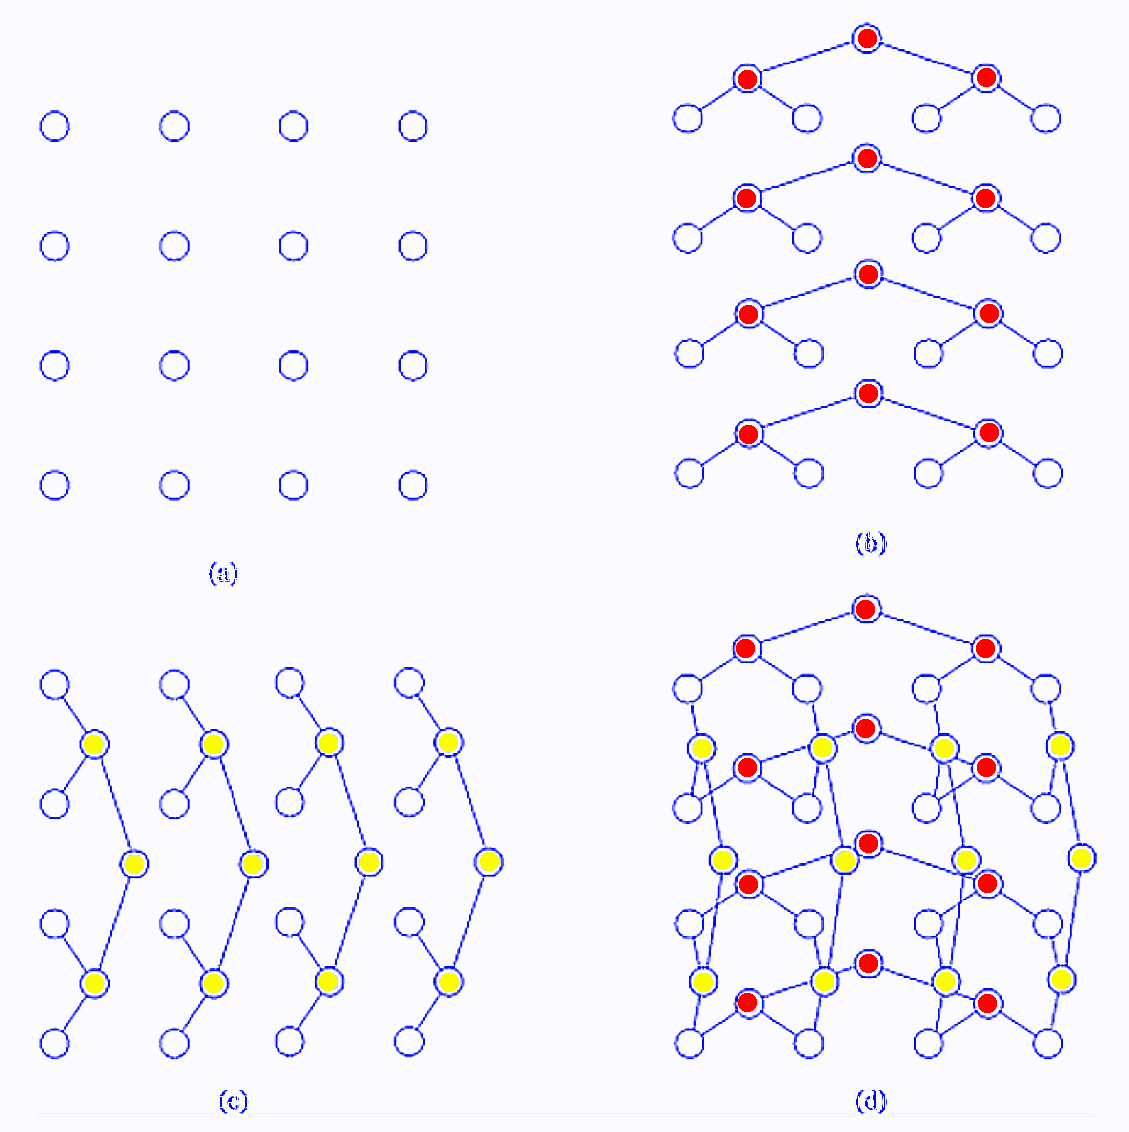
\includegraphics[width=10cm]{images/gda}
  \caption{Grille d'arbre 2-D construite sur une grille $N \times N$ avec N = 4 (a) à laquelle on connecte 4 arbres binaires horizontaux (b) et 
  4 arbres binaires verticaux (c) pour obtenir la grille d'arbres (d).}
  \label{fig:gda}
\end{figure}
\subsection{Les grilles d'arbres}

\paragraph{Définition d'une grille d'arbre bidimensionnelle :}
Une grille d'arbre bidimensionnelle, Mesh Of Trees en anglais ou MOT en abrégé, est construite à partir d'une grille
bidimensionnelle reliée par des arbres binaires verticalement et horizontalement comme illustré figure \ref{fig:gda}.
Les noeuds de la grille constituent les feuilles des arbres. On a donc $2N$ arbres de profondeur $p = \log_2(N) = 2$.
Chacun des $2N$ arbres est composé de $(N-1)$ noeuds internes et de $N$ feuilles. On a donc un nombre total de noeuds dans la grille
d'arbres égal à la somme des noeuds de la grille $N \times N$, soit $N^2$ et du nombre total des noeuds ajoutés par les arbres, soit $2N(N-1)$. 
Une grille d'arbres $N\times N$ est donc composée de $3N^2 - 2N$ noeuds.



\paragraph{Diamètre d'un arbre binaire: } Le diamètre est la distance ``diagonale'' entre le noeud supérieur gauche et inférieur droit. La géométrie
carrée implique que cette distance est le double de la distance qui sépare le noeud supérieur gauche et le noeud inférieur gauche. Or ces 2
noeuds sont les feuilles d'un arbre binaire qui compte N feuilles donc dont le diamètre est $D = 2p = 2\log_2(N)$. \textbf{Le diamètre d'une grille d'arbre}
est donc : \[D' = 4\log_2(N)\] 

\paragraph{Bissection d'une grille d'arbres : } La figure \ref{fig:gda} (c) montre qu'en déconnectant les N = 4 racines des arbres verticaux, 
on aboutit à deux sous-réseaux de même taille si on affecte une fois sur deux les noeuds racines ainsi déconnectés au
sous-réseau supérieur puis au sous réseau inférieur. \textbf{La bissection est donc N}.

\paragraph{Bilan : } Les grilles d'arbres sont des architectures performantes car elles jouissent à la fois d'un diamètre faible, donc de connexions 
plus rapides et directes, et d'une bissection élevée, donc d'une connectivité élevée entre deux parties de la structure. 
Ce qui implique un effet ``goulot d'étranglement'' moins important que dans d'autres architectures.
Elles sont en particulier plus efficace que les grilles ou les arbres simples.




\subsection{Implémentation du produit matrice-vecteur sur une grille d'arbres : }

On suppose qu'on dispose d'une grille d'arbres $N \times N$ sur laquelle on cherche à effectuer le produit matrice-vecteur Y = AX où $A = (a_{ij})$, $X = (x_i)$
et $Y=y_j$ avec $0\leq i,j\leq N-1$. 


\begin{enumerate}
 \item On introduit $x_i$ par la racine de l'arbre horizontal $i$ non représenté sur la figure \ref{fig:gda2}(b), $0\leq i\leq N-1$. 
 \item Les $x_i$ sont transmis aux feuilles au travers des arbres horizontaux de telle 
 sorte que chaque feuille de l'arbre de la ligne $i$ 
 reçoit $x_i$ à l'étape $\log N$.
 \item On introduit $(a_{ij})$ dans la feuille $(i,j)$ via les entrées $I_i$ à l'étape $\log N$. 
 \item La feuille $(i,j)$ peut alors calculer le produit $a_{ij}x_j$.
 \item Les résultats sont sommés vers la racine des arbres verticaux.
\end{enumerate}



\begin{figure}[htp]
  \centering
  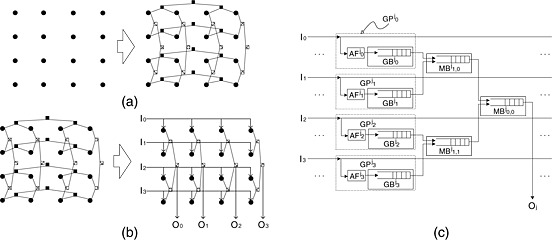
\includegraphics[width=15cm]{images/gda2}
  \caption{Grille d'arbres pour illustrer le principe du calcul d'un produit matrice-vecteur.}
  \label{fig:gda2}
\end{figure}


Après $2\log N$ étapes, la valeur \[y_i = \sum_{j=1}^{N} a_{ij}x_j\] est disponible dans 
la racine de la $i^{eme}$ colonne désignée par $O_i$ sur la figure \ref{fig:gda2} (b). 

\chapter{Les hypercubes}
\label{sec:unchapitre}

Lorem ipsum dolor sit amet, consectetur adipiscing elit. Sed non risus. Suspendisse lectus tortor, dignissim sit amet, adipiscing nec, ultricies sed, dolor. Cras elementum ultrices diam. Maecenas ligula massa, varius a, semper congue, euismod non, mi. Proin porttitor, orci nec nonummy molestie, enim est eleifend mi, non fermentum diam nisl sit amet erat. Duis semper. Duis arcu massa, scelerisque vitae,  convallis sollicitudin purus. Praesent aliquam, enim at fermentum mollis, ligula massa adipiscing nisl, ac euismod nibh nisl eu lectus. Fusce vulputate sem at sapien. Vivamus leo. Aliquam euismod libero eu enim. Nulla nec felis sed leo placerat imperdiet. Aenean suscipit nulla in justo. Suspendisse cursus rutrum augue. Nulla tincidunt tincidunt mi. Curabitur iaculis, lorem vel rhoncus faucibus, felis magna fermentum augue, et ultricies lacus lorem varius purus. Curabitur eu amet. Encore une citation \cite{Cadambe2008}.

\begin{figure}[htp!]
  \centering
  \setlength\figureheight{7cm}
  \setlength\figurewidth{9cm}
  % This file was created by matlab2tikz v0.2.2.
% Copyright (c) 2008--2012, Nico Schlömer <nico.schloemer@gmail.com>
% All rights reserved.
% 
% 
% 

% defining custom colors
\definecolor{mycolor1}{rgb}{0,0.75,0.75}

\begin{tikzpicture}

\begin{axis}[%
view={0}{90},
width=\figurewidth,
height=\figureheight,
scale only axis,
xmin=2, xmax=4.5,
xlabel={$\eta$},
xmajorgrids,
ymin=0.5, ymax=1,
ylabel={$d_{\text{min}}^2$},
ymajorgrids,
legend cell align=left,
legend style={align=left}]
\addplot [
color=black,
dashed,
mark=asterisk,
mark options={solid}
]
coordinates{
 (2,1)(2.1,1)(2.2,1)(2.3,1)(2.4,1)(2.5,1)(2.6,0.937749781479547)(2.7,0.890900393128398)(2.8,0.864988513955105)(2.9,0.827013168393703)(3,0.811347612650328)(3.1,0.792559278041243)(3.2,0.765840563467819)(3.3,0.749680961469385)(3.4,0.741947149227874)(3.5,0.740609493518419)(3.6,0.732128087463441)(3.7,0.717775843626632)(3.8,0.699687461812158)(3.9,0.685018622769455)(4,0.673439611642851)(4.1,0.664624248264608)(4.2,0.658255928882634)(4.3,0.641702335270489)(4.4,0.608326504614558)(4.5,0.580489221369454) 
};
\addlegendentry{$\alpha\text{ =  0\%}$};

\addplot [
color=black,
dashed,
mark=x,
mark options={solid}
]
coordinates{
 (2,1)(2.1,1)(2.2,1)(2.3,1)(2.4,0.958561324724996)(2.5,0.900812804739278)(2.6,0.859608621629443)(2.7,0.828484932127753)(2.8,0.812298837741994)(2.9,0.778916291864501)(3,0.758500630955482)(3.1,0.748375165853317)(3.2,0.745960208532468)(3.3,0.738441167434538)(3.4,0.715506361296671)(3.5,0.696927131434508)(3.6,0.682276848692725)(3.7,0.671128156410174)(3.8,0.663062783265717)(3.9,0.657680299791254)(4,0.621142740976429)(4.1,0.589786339121755)(4.2,0.564530571776849)(4.3,0.54483432747474)(4.4,0.53008799514765)(4.5,0.519641830384595) 
};
\addlegendentry{$\alpha\text{ = 10\%}$};

\addplot [
color=black,
dashed,
mark=triangle,
mark options={solid}
]
coordinates{
 (2,1)(2.1,1)(2.2,1)(2.3,0.966145915091813)(2.4,0.907589260275562)(2.5,0.862273165052718)(2.6,0.833762738286283)(2.7,0.797262289343802)(2.8,0.774689700869446)(2.9,0.763077871790574)(3,0.759584455148894)(3.1,0.735410358863577)(3.2,0.713220246811223)(3.3,0.695713299974315)(3.4,0.682371019886023)(3.5,0.672682085917092)(3.6,0.6661550402729)(3.7,0.644666127799479)(3.8,0.610083129739041)(3.9,0.582172698611821)(4,0.560333265725228)(4.1,0.543883933286703)(4.2,0.532098369213191)(4.3,0.524242326405)(4.4,0.519608701974017)(4.5,0.517545187250875) 
};
\addlegendentry{$\alpha\text{ = 20\%}$};

\addplot [
color=black,
dashed,
mark=triangle,
mark options={solid,,rotate=180}
]
coordinates{
 (2,1)(2.1,1)(2.2,0.995488894312993)(2.3,0.930050749246739)(2.4,0.882604857341179)(2.5,0.840148695151764)(2.6,0.807621264874927)(2.7,0.787889977099099)(2.8,0.777972678915356)(2.9,0.750463202108443)(3,0.726620292578349)(3.1,0.707917379352703)(3.2,0.693763185722015)(3.3,0.683575144048861)(3.4,0.676795290182409)(3.5,0.663350261880571)(3.6,0.627666127013326)(3.7,0.598755039468926)(3.8,0.575986310488554)(3.9,0.558651995817327)(4,0.546003746104731)(4.1,0.537291509323841)(4.2,0.531798375059385)(4.3,0.528867181690889)(4.4,0.527917002741411)(4.5,0.528450017604181) 
};
\addlegendentry{$\alpha\text{ = 30\%}$};

\addplot [
color=black,
dashed,
mark=o,
mark options={solid}
]
coordinates{
 (2,1)(2.1,1)(2.2,1)(2.3,1)(2.4,1)(2.5,0.995096871086856)(2.6,0.937749790013923)(2.7,0.890900391028178)(2.8,0.864988509535523)(2.9,0.827013167946275)(3,0.811347609462027)(3.1,0.79255927917077)(3.2,0.765840564829299)(3.3,0.749680963181722)(3.4,0.741947149533667)(3.5,0.740609492450166)(3.6,0.732128080624777)(3.7,0.71777584554089)(3.8,0.699687463368726)(3.9,0.681193180471954)(4,0.640212533267028)(4.1,0.617585040920557)(4.2,0.608519007405809)(4.3,0.608298095410932)(4.4,0.608326494076335)(4.5,0.580489212682311) 
};
\addlegendentry{Mazo};

\end{axis}
\end{tikzpicture}%
  \caption{Exemple de courbe TikZ.}
  \label{fig:courbe-tikz}
\end{figure}

\section{Implémentation du tri par fusion}
Lorem ipsum dolor sit amet, consectetur adipiscing elit. Sed non risus. 

\subsection{Quelques détails sur cette méthode}
Lorem ipsum dolor sit amet, consectetuer adipiscing elit. Morbi 

\subsection{On n'est jamais très fort pour ce calcul}
Lorem ipsum dolor sit amet, consectetuer adipiscing elit. 

\begin{align}
H_{m,n,p,q} &= \DPR{\rproto_{p,q}}{\OP{H} \tproto_{m,n}}\\
&= \iint\limits_{\SET{R}^2} S_{\OP{H}}(f,\tau) \DPR{\rproto_{p,q}}{\OP{U}_{f,\tau} \tproto_{m,n}} \ud f \ud \tau.
\end{align}

\section{Implémentation d'autres algorithmes}
Lorem ipsum dolor sit amet, consectetur adipiscing elit. 
%%% Local Variables: 
%%% mode: latex
%%% TeX-master: "isae-report-template"
%%% End: 

\appendix

\bibliographystyle{authoryear-fr}
\bibliography{references}

\clearpage

%%%%%%%%%%%%%%%%
%%% Abstract %%%
%%%%%%%%%%%%%%%%

% \thispagestyle{empty}
% 
% \vspace*{\fill}
% \noindent\rule[2pt]{\textwidth}{0.5pt}\\
% {\textbf{Résumé ---}}
% Lorem ipsum dolor sit amet, consectetur adipiscing elit. Sed non risus. Suspendisse lectus tortor, dignissim sit amet, adipiscing nec, ultricies sed, dolor. Cras elementum ultrices diam. Maecenas ligula massa, varius a, semper congue, euismod non, mi. Proin porttitor, orci nec nonummy molestie, enim est eleifend mi, non fermentum diam nisl sit amet erat. Duis semper. Duis arcu massa, scelerisque vitae, consequat in, pretium a, enim. Pellentesque congue. Ut in risus volutpat libero pharetra tempor. Cras vestibulum bibendum augue. Praesent egestas leo in pede. Praesent blandit odio eu enim. Pellentesque sed dui ut augue blandit sodales. Vestibulum ante ipsum primis in faucibus orci luctus et ultrices posuere cubilia Curae; Aliquam nibh. Mauris ac mauris sed pede pellentesque fermentum. Maecenas adipiscing ante non diam sodales hendrerit. Ut velit mauris, egestas sed, gravida nec, ornare ut, mi. Aenean ut orci vel massa suscipit pulvinar. Nulla sollicitudin. Fusce varius, ligula non tempus aliquam, nunc turpis ullamcorper nibh, in tempus sapien eros vitae ligula. Pellentesque rhoncus nunc et augue. Integer id felis.
% 
% {\textbf{Mots clés :}}
% Lorem ipsum dolor sit amet, consectetur adipiscing elit. Sed non risus. Suspendisse lectus tortor.
% \\
% \noindent\rule[2pt]{\textwidth}{0.5pt}
% \begin{center}
%   ISAE\\
%   10, avenue Édouard Belin\\
%   BP 54032\\
%   31055 Toulouse CEDEX 4
% \end{center}
% \vspace*{\fill}

\end{document}